%% question-7.tex
%%

%% ==============================
\subsection{Modélisation du concept de déclaration}
\label{sec:question7}
%% ==============================

La classe \emph{Déclaration} (Figure \ref{fig:program}) est raffinée dans la figure \ref{fig:declaration}. Dans cette figure, nous avons conservé les classes \emph{Named} et \emph{Programme} afin de faciliter la lecture du diagramme.

\begin{figure}
	\centering
	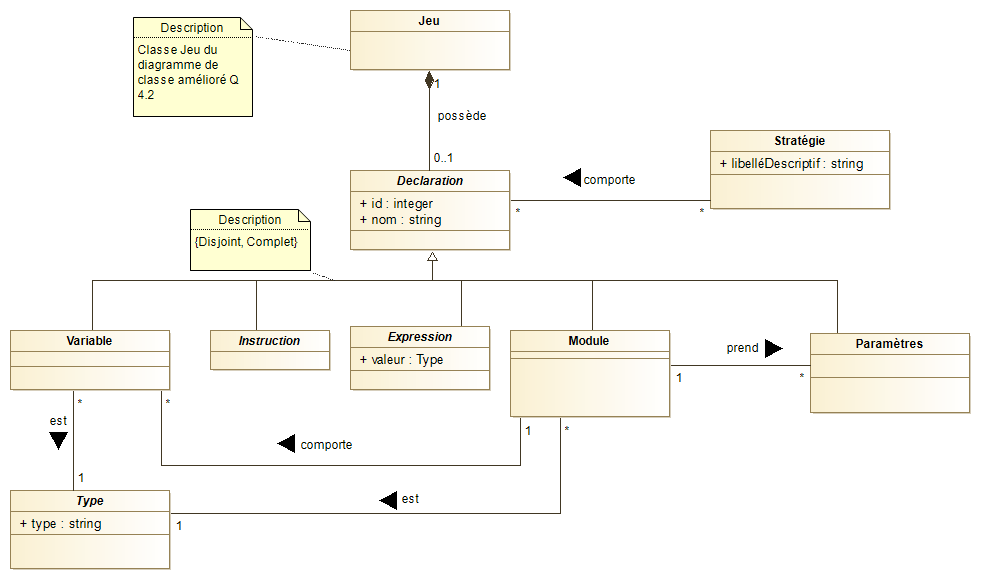
\includegraphics[width=500pt]{assets/class__Declaration}
	\caption{Diagramme de classe d'une déclaration}
	\label{fig:declaration}
\end{figure}


